\section{Authentication}

Authentication is the process of proving a claim or an assertion.
Today the most common application of authentication is in information security systems, however the methods of authentication are not limited to computer science and are also used in fields of archeology, anthropology and others.
\bigskip
\newline
In information systems authentication is used for establishing access between restricted system resources and users through digital identities.
Government and international institutions have developed guidelines for managing digital identities and authentication processes.
\bigskip
\newline
We focus on password based authentication, its security assumptions and tools used in practical applications for increasing security and minimising damage in security breaches.

\subsection{Authentication in Information Security}
Authentications is a method used in information security to manage access between restricted system resources and an external user wishing to access them.

As defined in RFC-4949 \cite{shirey2007internet}, authentication is "the process of verifying a claim that a system entity or system resource has a certain attribute value."
This is a broad definition, and it most frequently applies to the verification of users identity (e.g at login), however assertions can be made and verified about any subject or object.
The process of authentication is done in two parts, \textit{identification} and \textit{verification}.

\paragraph{Identification} Presenting an identifier to the authentication system, that establishes the entity being authenticated.
In common user authentication systems this is a username or an email verified in the registration process. 
The identifier needs to be unique for the entity it identifies.
The identity of the subject/object can also be pre-determined, so this process is not necessarily visible to the user.

\paragraph{Verification} Presenting or generating authentication information that can be used to verify the claim.
Commonly used authentication information are passwords, one-time tokens, digital signatures.

\subsection{The NITS Model for Digital Identity}

Digital Identity Guidelines \cite{grassi2017} published by the National Institute of Standards and Technology (NIST) describes a simple digital identity model, that provides a generic authentication framework.

The process has distinct steps of \textit{Enrolment} and \textit{Authentication}.

\begin{figure}[h]
	\centering
	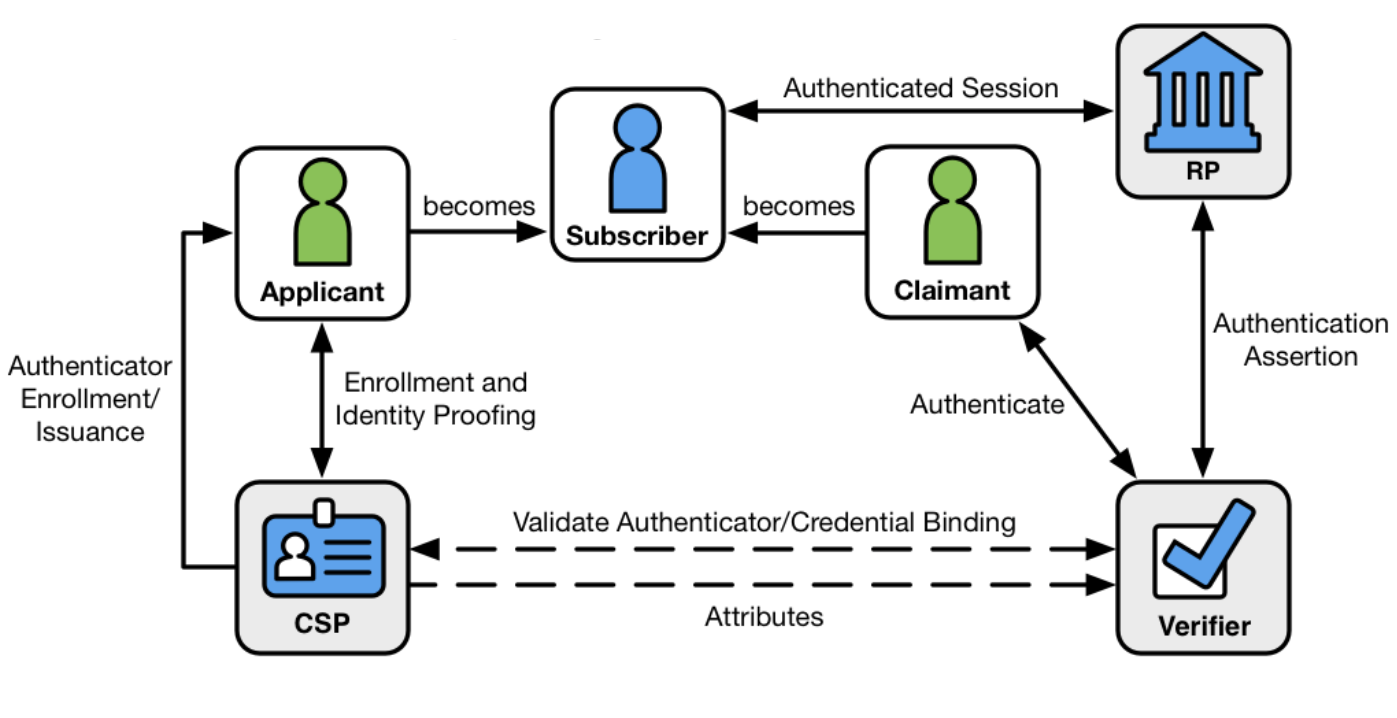
\includegraphics[width=13cm]{images/NIST_digital_identity_model}
	\caption{NITS Digital Identity Model}
	\label{fig:NIST-digital-identity-model}
\end{figure}

\paragraph{Enrolment}

The enrolment is a process where an \textit{applicant} becomes a \textit{subscriber} after being successfully \textit{proofed} by a \textit{CSP}.
The subscriber is issued a \textit{credential} and one or more \textit{authenticators}.
\bigskip
\newline
A common application of this process is \textit{user registration} on websites.

\paragraph{Authentication} 
The \textit{claimant} begins authentication with the \textit verifier by sharing the credential and the authenticators. The \textit verifier validates binding between the credential and authenticators with the \textit CSP.
An authenticated connection is established between the \textit subscriber and the \textit RP after and assertion is provided by the \textit CSP or the \textit verifier to the \textit RP.
\bigskip
\newline
A common application of this is \textit{user login} on websites.

\paragraph{Note on delegation of roles}
In the digital identity model \ref{fig:NIST-digital-identity-model} roles of \textit CSP, \textit verifier and \textit RP are distinct in their responsibility. 
In practice however all these roles can be performed by a single party (e.g any website with native registration and login).

In OAuth2's \cite{hardt2012oauth} authentication layer, the resource owner has the roles of \textit applicant, \textit claimant and \textit subscriber. The authorisation server has the roles of \textit CSP and \textit verifier. The OAuth2 client has the role of the \textit RP.

\subsection{Authentication Factors}

As described in \cite{council2005authentication} authentication systems can rely on three distinct "factors".

\begin{itemize}
	\item \textbf{Knowledge factors} - Something the user \textbf{knows} (e.g, password, security question, PIN)
	\item \textbf{Ownership factors} - Something the user \textbf{owns} (e.g, ID card, security tokens, mobile devices)
	\item \textbf{Inherence factors} - Something the user \textbf{is} or \textbf{does} (e.g, static biometrics - fingerprints, retina, face. dynamic biometrics - voice patterns, typing rhythm)
\end{itemize}

\paragraph{Strong authentication} As defined by governments and financial institutions \cite{schaeffer2010national, ecb2013recommendations}, secure authentication is based on two or more authentication factors. 
This is also referred to as \textit{multi-factor authentication}.

\newpage
\section{Password Authentication}

Passwords are one of the most common and oldest forms of user authentication. 
They were first used in computers at MIT in the mid-60s \cite{mcmillan2012password}, but their use goes back to ancient times in the Roman military.

\subsection{Authentication Model}

% High level arch
Password based authentication is a simple efficient authentication model, based on a shared secret between a user and a system. 
The secret (password) is often used in a combination with a user ID. 
The password itself is a set of characters memorised by the user, and inputted via a keyboard.

Using NIST Digital Identity Guidelines terminology \cite{grassi2017}, the password and the user ID are issued as a credential and an authenticator to the applicant after successful enrolment by the CSP.
A claimant then uses the credentials to authenticate with the verifier, as to establish an authenticated session with the RP.


% Security considerations
\subsection{Security}

The threat model needs to account for a variety of attack vectors like network conditions (data confidentiality), integrity of host systems.
Some attack vectors are specific to password based authentication, with how passwords are chosen, handled and stored.

Common password based authentication systems over the web rely on the user sending a plain-text password over a secure HTTPS connection, and the server verifying the password.

The simplicity that makes passwords effective is also a big security downside.
Because passwords are supposed to be memorised and the proliferation of different websites requiring them, users tend to pick password that are easier to remember and reuse passwords across different websites \cite{conklin2004password}.
Many websites also don't properly handle and store passwords, allowing attackers to "learn" about users passwords in case of a security breach.

\subsubsection{Security Attacks}
Attacks can be according to NIST \cite{grassi2017} classified as \textit online or \textit offline, based on wether the attacker is directly interacting with an authentication system or not.

\paragraph{Online Password Attack} A form of an \textit{active attack}, where an attacker is attempting bypass authentication by directly interacting with the system.
These attacks are usually very noisy, making it easy for an authentication system to detect an attack is happening, and prevent it.
This makes online attacks much less effective than offline ones.

Popular methods of online password attacks are \textit{password spraying} and \textit{credential stuffing}, both of which utilise information from data breaches, like username  and password combinations, or lists of most commonly used passwords. %TODO: Maybe add mitigation strategies

\paragraph{Offline Password Attack} A form of a passive attack where an attacker is able to analyse data in a system he controls. Data was obtained by the attacker by either theft of file, eavesdropping an authentication protocol or a system penetration.

\textit{Password cracking} is method of extracting user credentials from data used by the authentication system to verify users credentials.

The success of password cracking is generally determined by two factors, that influence the time required to guess the password.

\subparagraph{Password Handling}
Password handling describes how passwords are stored at rest and used in the verification process.

A naive system might store the passwords or password-equivalent data in plain text and compare them for verification, while simple this system is insecure as user credentials directly are exposed with any unauthorised access.

A common approach today is to use methods of \textit{password hashing} to derive a password digest that is then stored in the database. 
When verifying the password is hashes again, and the digests are compared.

Using pure hashing functions like SHA family is discouraged because they designed to run fast and can be accelerated with ASIC chips, making them vulnerable to pre-computed hash tables.
A better solution are password key-derivation functions. 
Algorithms utilising hash functions designed with the purpose of being both time-consuming and memory-hard, examples of such tools are Argon2 \cite{biryukov2016argon2}, Scrypt \cite{percival2016scrypt} and Balloon \cite{boneh2016balloon}.
Using an extra value called \textit{salt} \cite{hornby2016salted} prevents attacks with pre-computed hash tables.
Because salt is stored alongside password hashes, systems sometimes also utilise a third value called \textit pepper, which is the same for all passwords, but stored in a different place from the salt.


\subparagraph{Password Strength}
Measure of information entropy and the difficulty of the password being guesses or brute-forced.
Re-using passwords greatly undermines password strength and is what attacks like credential stuffing rely on.
Have I Been Pwned \cite{hunt2021have} catalogs 613,584,248 passwords recovered from data breaches, while CrackStation \cite{hornby2019password} lists a collection of 1,493,677,782 words used for password cracking.